\documentclass[linenumbers]{aastex7}
\newcommand{\vdag}{(v)^\dagger}
\newcommand\aastex{AAS\TeX}
\newcommand\latex{La\TeX}

\begin{document}

\title{Calibration of Analog to Digital Converters with Considerations from DNL and INL}

\author{Renee Nichols}
\affiliation{Department of Physics, University of California Santa Cruz, Santa Cruz, CA 95060}
\email[show]{rejnicho@ucsc.edu}  

\author{Adrian Shestakov}
\affiliation{Department of Physics, University of California Santa Cruz, Santa Cruz, CA 95060}
\email[show]{ashestak@ucsc.edu}  

\author{Duncan Wood}
\affiliation{Department of Physics, University of California Santa Cruz, Santa Cruz, CA 95060}
\email[show]{duwood@ucsc.edu}  

\author{Steven Ritz}
\affiliation{Department of Physics, University of California Santa Cruz, Santa Cruz, CA 95060}
\email[show]{sritz@ucsc.edu}  

\begin{abstract}
    This work outlines a calibration of Analog to Digital Converters (ADCs) using a differential nonlinearity informed method.
This method was developed and applied for use in Rubin Observatory's LSST Camera. 
We use two dataset types from the LSST Camera EO testing to verify the method we call the cumulative binning method. 
The method examines the long range behavior of the ADC and places the bin edges according to the probability distribution function (PDF). 
The calibrated results showcase the individual periodic, braided structure of each ADC and recovers important quantities of the ADCs, including differential and integral nonlinearity which fall within specifications from the manufacturer, Analog Devices (\cite{AnalogDevices}). 


\end{abstract}

\keywords{\uat{Astronomical Instrumentation}{799} --- \uat{Calibration}{2179} --- \uat{Ground-based astronomy}{686} --- \uat{Wide-field telescopes}{1800} --- \uat{Optical astronomy}{1776}}

\section{Introduction}
\label{sec: Motivations}

The Vera C. Rubin Observatory, located on Cerro Pachón, Chile, is the next generation of ground based, optical astronomy. 
The Observatory's Simonyi Survey Telescope is a modified Paul-Baker design with a 8.4m primary mirror corresponding to a 9.6 square degree field of view. 
Rubin Observatory, with the LSST Camera, begins the Legacy Survey of Space and Time (LSST) this year -  a wide, fast, deep (WFD) survey. 
Over the course of the survey, the LSST will capture over 20,000 square degrees of the southern sky. 
The survey design includes 30s visit times to each sky pointing.
The depth is created by revisiting each pointing over 100 times over the 10 year survey in the 6 broadband optical filters, ugrizy. 
Together, the LSST project aims to examine 4 central science themes: Probing Dark Energy and Dark Matter, Taking an Inventory of the Solar System, Exploring the Transient Optical Sky, and Mapping the Milky Way (\cite{Ivezic2019}).

The primary instrument in Rubin Observatory is the LSST Camera, the largest digital camera ever constructed.
The camera features 3.2 gigapixels arranged over 189 science grade charge coupled devices (CCDs) manufactured by two vendors Teledyne (e2V) and Imaging Technology Laboratory (ITL). 
Each pixel has a physical size of 10\textmu m x 10\textmu m and a plate scale of 0.2"x0.2" (\cite{Doherty2014}).
Groups of 9 CCDs are arranged as 3x3 rafts, with subgroups of 3 CCDs connecting to a single readout electronic board (REB) (\cite{OConnor2016, Lopez2018}). 
The focal plane consists of a 5x5 array of these rafts, with the partial corners rafts consisting of a single wavefront sensor and 2 guiding sensors (\cite{Arndt2010, Gilmore2008}). 
Together, this design comprises the entire focal plane.

CCDs are a common choice of imaging sensor, used in precursor camera systems such as Hubble's Wide Field Camera (\cite{Wyckoff1993}), Dark Energy Survey's DECam (\cite{Flaugher2015}), and Subaru's Hyper-Suprime Camera (\cite{Miyazaki2018}). 
The specific CCDs used for the LSST Camera are 100\textmu m thick, a thickness selected to maximize infrared response and minimize charge diffusion(\cite{OConnor2006}).  
To minimize observation dead time and achieve the desired 2s read out, each CCD is segmented into 16 channels of 1 million pixels. 
Each of the 3024 channels, or amplifiers, is read out in parallel with its own readout electronics (\cite{Lange2024}). 

Before integration, the CCDs were characterized through extensive testing at the vendors, Brookhaven National Lab (BNL), and SLAC National Accelerator Laboratory to understand quantities such as quantum efficiency, bright and dark defects, and charge transfer inefficiencies (CTE) (\cite{Kotov2016, Doherty2014}).
The camera was later assembled at SLAC, and the full focal plane was studied in electro optical (EO) testing at SLAC to measure critical characteristics such as the bias, saturation, and linearity, (\cite{Roodman2024}) for each CCD.
The voltages and timing electronics for the entire system have also been optimized for operations (\cite{Utsumi2024}). 
Further optimization was completed at the Rubin Observatory cite for on sky operations (\cite{Antilogus2025}). 

All calibrations and studies are integrated into an instrument signature removal (ISR) pipeline (\cite{PlazasMalagon2025}). 
One necessary but previously not included calibration is the Differential Nonlinearity (DNL) correction due to the analog to digital converters (ADCs).
This calibration yields a look-up table (LUT), which removes the internal structure of the ADCs to recover the pre digitized signal levels, more on ADC function in Section \ref{sec: DNL_INL_Def}. 
Previous work from the Hubble Wide Field Camera demonstrates consideration for the ADC correction but does not outline such a method for its computation and correction (\cite{Wyckoff1993}).
In this work we will motivate and produce the missing DNL ADC calibration for the 3024 ADCs in the LSST Camera.
Our findings demonstrate each Analog Devices 18-bit, 1 MSPS PulSAR ADC (\cite{AnalogDevices}) in the LSST Camera falls within the specifications from the manufacturer. 

The cumulative binning method is built and examined in the following sections. 
Section \ref{sec: Motivations} defines differential nonlinearity and integral nonlinearity, specifies the criteria for calibrating data, and describes the data preparation process. 
Section \ref{sec: Cummulative binning} motivates the cumulative binning method via the probability distribution function (PDF) of the signal incoming to the ADCs and demonstrates how the data are applied to the model. 
The results of the method, including highlights of differences due to calibrating run type are detailed in Section \ref{sec:results}.
Section \ref{sec:Future} details how to apply this calibration, and includes a sample look-up table (LUT) for one ADC. 
Finally, the appendices note additional information learned from this calibration to guide the reader in conducting a calibration themselves. 

\subsection{Definition of Differential and Integral Nonlinearity}
\label{sec: DNL_INL_Def}

An analog to digital converter (ADC) is an electronic component which converts a continuous signal, such as a voltage, to an integer value corresponding to that amount. 
The digital signal is measured in integer analog to digital units (ADU). 
Each ADC has an unique structure which maps specific voltages to ADU, meaning specific ranges of voltage yield the same ADU. 
The limits for the voltage mapped to each ADU are called the edges, with the left edge specifying the lower bound and the right edge the upper bound. 
The difference between the two edges is called the ADC binwidth, and is a unique value for each ADC and each ADC bin. 
For the 3024 18-bit ADCs used on the LSST Camera, this corresponds to \(3024*2^{18}\) unique bin edges. 

\begin{figure}[t]
    \centering
    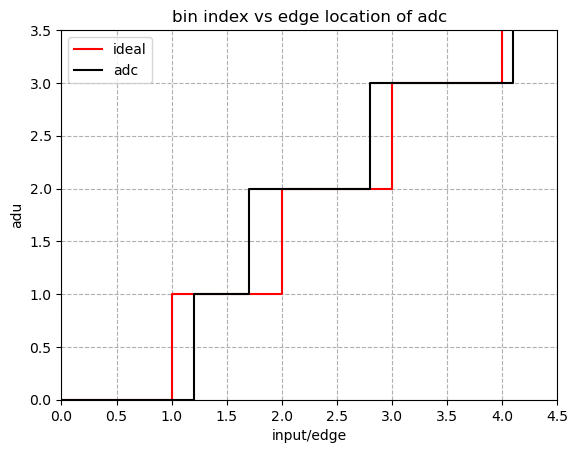
\includegraphics[width=0.5\linewidth]{ADCModel.png}
    \caption{A schematic demonstrating how the analog to digital converter ideally works (red), and its true fabricated behavior (black). On the y axis is the ADU value recorded by the ADC, which has integer values. On the x axis is the edge of the ADC, or the left and right edges of the bin which maps to a given ADU. As tracked along the red, an ideal ADC has bins with integer edges which map to corresponding ADU. The black shows a simulated true ADC, which has left and right edges that deviate from the ideal, but still maps to a single ADU.}
    \label{fig:idealADC}
\end{figure}


As seen in Figure \ref{fig:idealADC}, both the ideal ADC (red) and the mock ADC (black) yield integer spaced ADU steps on the y axis. 
This corresponds to the output of the ADC.
The input or voltage the ADC is converting is along the x axis, and demonstrates the difference between the ideal and mock ADC. 
In the ideal ADC the edges of the input are integer values, while in the mock ADC the edges are reals. 
These non-integer edges can yield non uniform bin sizes which are not present in the ideal ADC, but are expected in a true ADC.

The non uniform bin sizes are characterized as two types of nonlinearity: differential nonlinearity (DNL) and integral nonlinearity (INL). 
DNL is the deviation of a bin's width from that of an ideal bin width and is defined exactly as
\begin{equation}
DNL & = w_{ideal} - w_{ADC} = 1- w_{ADC}  
\label{eq: DNL}
\end{equation}
where $w_{ideal}$ and $w_{ADC}$ are the ideal and true binwidths respectively, and $w_{ideal}$ = 1.  
The DNL can be computed for all ADC bins along the ADC. 
DNL values are typically on the order of $\pm$ 0.5, and any value greater than $\pm$ 1 indicates a skipped bin or code. 

Integral nonlinearity is the deviation of the middle of a bin from that of an ideal bin, which is denoted as
\begin{equation}
INL = m_{ideal} - m_{adc} 
\label{eq: INL}
\end{equation}
where $m_{ideal}$ is the midpoint of an ideal bin, and $m_{adc}$ is the midpoint of an ADC bin. 
The midpoint is calculated for each ADC bin with corresponding ADU.
For an ideal bin the midpoint is always  ADU+0.5. 
INL typically yields contributions from each bin on the order of $\pm$ 1. 

The manufacture of the ADCs used for the LSST Camera, Analog Devices, has a published specifications sheet detailing expected behavior of the ADCs. 
These include, no skipped bins, DNL between [-0.85, 1.5] with typical $\pm 0.5$, and INL between [-2,2] with typical $\pm 1$ (\cite{AnalogDevices}). 
We note these metrics provide valuable insight to the structure of the ADCs, and we will compare the results for the LSST Camera's ADCs to the manufacturer's criteria in Section  \ref{sec:results}. 

\subsection{Run Selection and Preparation}
\label{sec: RunSelPrep}

In order to understand the structure of the ADCs used in the LSST Camera, we must look at data digitized by those same ADCs. 
The data collected for the LSST Camera is arranged as collections of exposures, called runs. 
These runs, completed at SLAC and the summit during EO testing, are designed with specific calibrations and characterizations as their focus, which help inform ISR corrections(\cite{PlazasMalagon2025}).
For our calibration, we will use one readily available run type, a flat pair, and one specialty ramp run, numbered 13144 and 13549 respectively. 

In this section we will examine the requirements to use this data in order to conduct the calibration in Section \ref{sec: Cummulative binning}. 
These requirements include showing the entire dynamic range of the CCD as in Section \ref{sec:RangeADC}, rescaling data with variable density of information as in Section \ref{sec:RollingScaling}, and trimming exposures to remove edge effects in Section \ref{sec:Trimming}.

\subsubsection{Full Dynamic CCD range}
\label{sec:RangeADC}

The ADCs used in the LSST Camera are implemented to read the signal from the CCDs themselves. 
The bounds of the signal into the ADCs are directly related, by their gain, to the bias and saturation of the CCDs themselves.  
Due to the photoelectric conversion of light on the CCDs, a range of incident flux to the CCDs is necessary to look at the used range of the ADCs.
In our calibration we desire to examine all ADU codes received from the ADCs, which amounts to approximately 100k per ADC.  
We then search available datasets to fit this requirement.

The first dataset covering this range of ADU codes is a flat pairs run, 13144. 
When all exposures are compiled into a single histogram in counts per ADU, the behavior of the ADC can start to emerge.
Figure \ref{fig:13144Distributions} demonstrates a combined distribution for an example amplifier, R22S00C01.
This plot shows variations in the amount of signal present in each bin over the target range of the ADC.
The bin-to-bin deviations are two-fold. 
The most dramatic is the right skew of the signal, which corresponds to a high density of exposures with low exposure time, and therefore low ADU.
This structure is the result of the log-based flux sampling used for the flat pairs increasing the number of exposures in the low flux region. 
This is amplified by Poisson spreading of the signal about its mean, which broadens as a function of flux. 
This results in a two order of magnitude difference in the signal near bias as compared to saturation.
This difference will have to be scaled out in order to use this run for our ADC calibration, as discussed further in Section \ref{sec:RollingScaling}. 
On a smaller scale, we note the presence of local bin-to-bin deviations that denote the presence of DNL in the ADC, as seen in the upper portion of Figure \ref{fig:13144Distributions}. 

The second dataset which covers the dynamic range of the CCD is a specialty ramp run 13549. 
The ramp run was designed to look at the ADC signal without superimposed run structure.
This was accomplished by allowing the sensors to continue to integrate charge as the focal plane was read out, resulting in exposures with a base illumination plus a ramp upwards. 
This was repeated three times for each of the 78 exposure times, spaced 2.2s apart, to cover the flux range of the signal into ADC from the CCDs.
Our sample distribution for our reference amplifier is shown in Figure \ref{fig:13549Hist}.
We note the full range of the CCD is covered uniformly, and the presence of local bin-to-bin deviations from structural DNL in the ADC remains.  

\begin{figure}
    \centering
    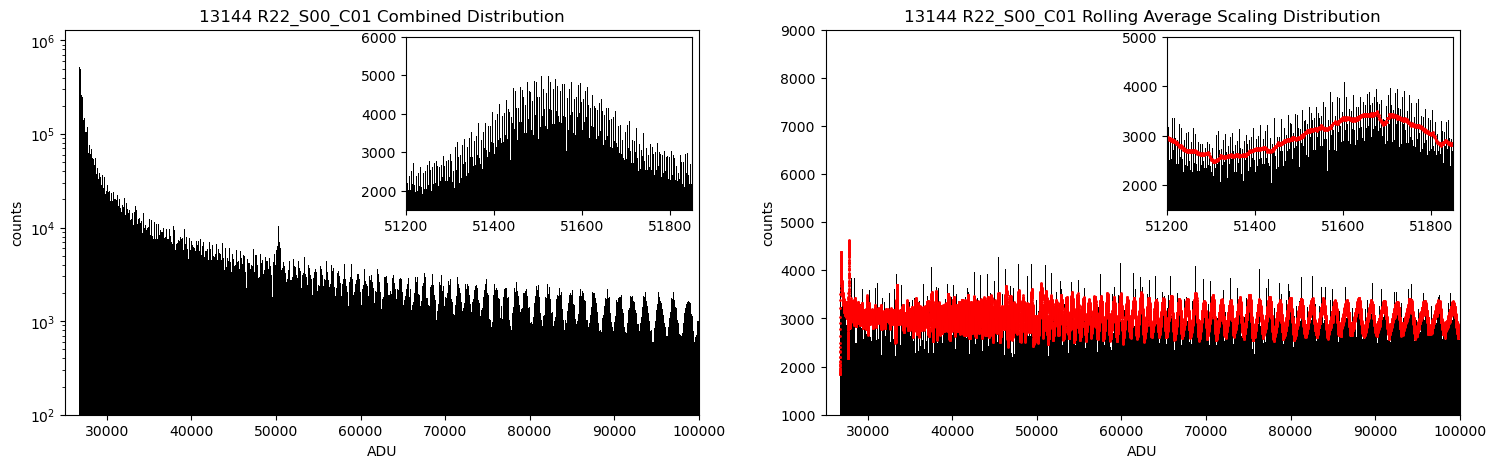
\includegraphics[width=1\textwidth]{13144rescaledmarch.png}
    \caption{The combined distribution of all exposures from a single amplifier, R22S00C01, from 687 flat pair in run 13144. On the left side is the distribution from the run itself. The distribution demonstrates a greater density of exposures in the sub-30,000 ADU region, yielding a distribution with counts more than two orders of magnitude greater than later higher-flux regions of the ADC. A second notable feature is the oscillatory peak-like behavior throughout the distribution. This is due to the exposures representing Poisson distributions of the photoelectric effect and adding many of these high mean Gaussian approximated Poisson distributions together. The upper plot zooms in on bin-to-bin behavior, showing that bin-to-bin there are small deviations of counts present as well as some patterned downticks every 128 counts, as discussed further in Section \ref{sec:results}. On the right above is a rolling average scale of the left distribution for the same amplifier. The scaling process is outlined in Section \ref{sec:RollingScaling}. Even after scaling, the bin to bin deviations remain.  In red is the output from a Savitzky-Golay filter with window size 33 and order 3. The deviations between the filter and the histogram directly demonstrate presence of DNL in the ADC.}
    \label{fig:13144Distributions}
\end{figure}


\subsubsection{Rolling Scaling Method}
\label{sec:RollingScaling}

For an ADC calibration, we seek to understand the substructure of the ADC itself, or how signal is expected to fall into each of the ADC bins. 
We call the distribution of ADU values for a given amount of light the probability distribution function (PDF).
This is how many pixels the amplifier will yield for each ADU value given some accumulated charge. 
We have no \textit{a priori} knowledge of this distribution and must infer it from the signal we receive from the ADC.
It is from this PDF that one can then determine the bin edge locations given the measured occupancy of each bin as in Section \ref{sec: Cummulative binning}. 

From the two runs used for this calibration, we see structural differences in the data density over the ADC range covered for the same amplifier. 
Figures \ref{fig:13144Distributions} and \ref{fig:13549Hist} highlight this difference, notably for lower ADU in Figure \ref{fig:13144Distributions} there are multiple orders of magnitude more signal in these bins as compared to Figure \ref{fig:13549Hist}. 
This structural difference, if not scaled out, will result in small bins (on average) with large DNL and an unstable (bin starting dependent) INL as seen in Appendix \ref{sec:Adrianmethod}. 

To prevent arbitrary substructure injection and to be able to use widely available flat pairs runs, we utilize a rolling scaling method on run 13144 to flatten the signal over the entire ADC range.
While the ramp run prevents needing this rescaling, it is not always practical to request a special run of exposures for this calibration given the time necessary for the run.
By using a rolling scaling method, we can prepare the flat pairs to minimize the skew of their distribution and create a pseudo-flat distribution for the ADC calibration. 

Since the earliest, lowest-flux region of the ADC is most peaked, it is necessary to have a method which preserves the inherent structure but also reduces the overall signal per bin in a way that is proportional to the original signal.
To scale the flat pairs due to the uneven density of exposures, we utilize a rolling mean scale method. 
For each window of 100 bins in the histogram we calculate the mean of the window, $\bar x_{i}$, with starting bin i
\begin{equation}
\label{eq: rollingmean}
\bar x_{i} = (\sum_{i}^{i+100}c_{i})/100
\end{equation}
where $c_{i}$ is the occupancy of the i-th bin. 
This is repeated for the each ADC bin. 
We justify the use of the window of size 100 in Section \ref{sec: BitFractions}, where we examine the data for DNL on order this or larger and find no notable features. 

Next we calculate the rescale value of each histogram bin $c_{i}^{*}$
\begin{equation}
\label{eq: rescaled}
c_{i}^{*} = (3000*c_{i})/ \bar x_{i}
\end{equation}
The value 3000 is selected as the average value of the distribution beyond 50k ADU. 
Amplification of signal is prevented by limiting the factor $3000/ \bar x_i \leq 1.$
The result of this scaling for the sample amplifier and run 13144 is shown as  the right plot in Figure \ref{fig:13144Distributions}. 
The plot clearly demonstrates an effective dampening of the low-flux region while maintaining bin-to-bin substructure as seen in the zoom portion of the right plot. 
An additional scaling method, a dynamic prescale method is described in Appendix \ref{sec:Dynamic Prescaling}. 

\subsubsection{Trimming}
\label{sec:Trimming}

Each of the combined histograms seen in Figures \ref{fig:13144Distributions} and \ref{fig:13549Hist} are the sum of many individual exposures. 
The histograms of these exposures themselves can also have structure, such as peaks of low signal near the bias level.
Upon further investigation, these low ADU peaks correspond to specific locations on the CCDs near the edges of the sensors. 
On these edge locations, the pixels have diverging electric fields causing the signal to be less than its true signal. 

To mitigate this issue, we examine trimming between 0 and 12 pixels from the edges of the CCD to remove this feature. 
Our testing demonstrated 2 pixels was sufficient in removing this feature.
For consistency we trim all exposures in both the ramp and flat pairs runs. 
The result of each trimmed exposure is then complied into a single histogram for the ADC calibration.
We note the histograms shown in Figures \ref{fig:13144Distributions} and \ref{fig:13549Hist} have been trimmed and are the distributions used in the calibration as in Section \ref{sec: Cummulative binning}. 

Trimming of images due to diverging edge effects can also be referred to a picture frame removal. 
The ISR corrections for LSST science image preparation also includes picture frame removal with requirements different from what we report here.

\begin{figure}
    \centering
    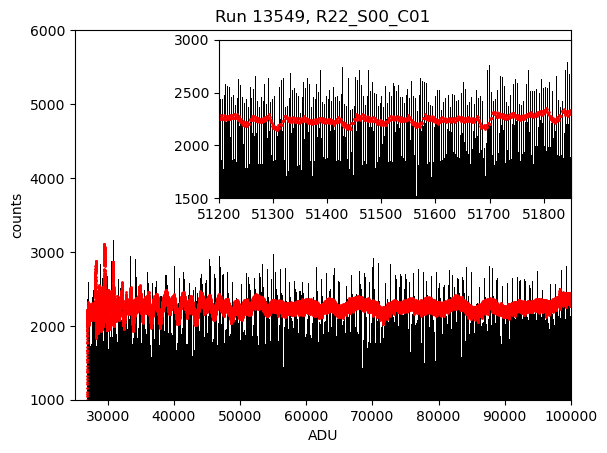
\includegraphics[width=0.5\linewidth]{13549Filter3.png}
    \caption{The combined distribution of all 234 exposures for a single amplifier, R22S00C01, in EO testing run 13549. Overlaid in red is the output from a Savitzky-Golay filter with window size 33 and order 3. Over the range of the ADC used, the signal in all bins remains relatively consistent. In the upper right portion of the plot is a zoomed-in section of the ADC demonstrating the oscillatory nature of the distribution as well as the deviations between the filter and the distribution, a sign of the DNL present in the ADC.}
    \label{fig:13549Hist}
\end{figure}

\section{Cumulative Binning Calibration}
\label{sec: Cummulative binning}

In this section we formally define the cumulative binning method for calibration of the ADCs. 
Section \ref{sec: Filter} motivates modeling an ideal ADC based on each dataset used in the calibration. 
This model ADC is based on a Savitzky-Golay filter and is related to the PDF in Section \ref{sec:PDFEdges}. 
Section \ref{sec:PDFEdges} will discuss the formal definition of the histogram distributions, as seen in Figures \ref{fig:13144Distributions} and \ref{fig:13549Hist}, and relate these to the probability distribution function (PDF).
The section then relates the PDF and histograms to determine the bin edges of the ADCs. 
Sections \ref{sec:Recommended start} and \ref{sec: SkippedBins} discuss where the calibration should start and how to check for skipped bins in the calibration. 
Finally, Section \ref{sec: Git} links to example python code with this calibration implemented. 

\subsection{Savitzky-Golay Filter}
\label{sec: Filter}

The histograms in Figures  \ref{fig:13144Distributions} and \ref{fig:13549Hist} demonstrate variable bin-to-bin occupancy in each ADC bin.
This is the inherent DNL structure of the ADC, and is unique for each ADC.
In order to compute the bin edges as in Section \ref{sec:PDFEdges}, we must model the bin occupancy for each ADC given no DNL. 
We want this model to represent the long range behavior of the ADC, such as our observed 128 bin low bins structure seen in Figure \ref{fig:13549Hist}, while minimizing bin-to bin deviations. 

From additional work on these ADCs, as noted in Appendix \ref{sec: BitFractions}, the DNL primarily occurs in bits 0 and 1. 
Therefore a model ADC without this DNL would need to smooth the behavior of the ADC on a scale larger than this DNL.
For our choice, we use a smoothing window size of 33, which is well beyond the 4 bit observed DNL. 
Applying  a Savitzky-Golay filter of order 3 and a window size of 33 we achieve the model ADC behavior without the low bit DNL we expect to recover. 
Additional types of filters could be employed for this task, and more details on selecting the filter type is discussed in the Appendix
\ref{sec:OtherFilters}. 

We overlay the filtered values (red) on the combined histograms for the flat pairs and ramp runs as seen in the right plot of Figure \ref{fig:13144Distributions} and Figure \ref{fig:13549Hist}.
Effectively, this demonstrates the preservation of long range behavior and smoothing on smaller scales. 
This filter allows us to relate the distributions and the filter to the PDF in Section \ref{sec: Cummulative binning}. 

\subsection{PDF definition and determination of ADC edges}
\label{sec:PDFEdges}


Given the preparation of the data from Section \ref{sec: RunSelPrep} and the filter from Section \ref{sec: Filter} we relate these pieces to the probability distribution function (PDF) alluded to before.
In the histograms, each count of ADU represents the number of times the signal has fallen between the left and right edge of its signal bin, described as
 \begin{equation}
c_i =  \int_{l}^{r} \varrho dx
\label{eq:pdfcounts}
\end{equation}
where l and r are the left and right edges of the ADC respectively, $\varrho$ is the pdf for the specific ADC, and $c_i$ is the count occupancy of ADU bin i. 
We also can determined the relationship between the filtered distribution values and the PDF,
 \begin{equation}
f_i =  \int_{x_i}^{x_{i+1}} \varrho dx
\label{eq:pdffilter}
\end{equation}
where $f_{i}$ is a filtered output for ADU bin i.
Since the filter models an ideal, no DNL ADC, the bin edges are exactly integers corresponding to the ADU reported by the ADC.
In this calibration the model is a Savitzky-Golay filter with a window size of 33 and order 3 as described in Section \ref{sec: Filter}. 
Using equation \ref{eq:pdffilter} as the description of the filter, we can utilize the fundamental theorem of calculus to examine how the PDF behaves over large regions of the ADC, 
\begin{equation}
F_{i}=\sum_{i=0}^{j} f_i= \int_{0}^{x_{j+1}} \varrho dx
\label{eq:fidef}
\end{equation}
where $F_i$ is the cumulative sum of the filtered values from bin 0 to bin j of the ADC. 
Examining the distribution of many of these cumulative sum terms $F_i$, one can see the gradual accumulation of PDF behavior for integer edges. 
To get the non-integer edge values, as necessary for the ADC calibration, we interpolate over many successive cumulative sums using a cubic spline function $\zeta$. 
This allows us to reform the integral of the observed distribution as
 \begin{equation}
c_i = \zeta(r) - \zeta(l)
\label{eq:countsspline}
\end{equation}
where $\zeta(l)$, $\zeta(r)$ are the values of the cubic spline at the left and right edge respectively for the ADU bin i.
To solve for the right edge, we rearrange eq. \ref{eq:countsspline}: 
 \begin{equation}
\zeta(r) = c_i + \zeta(l) 
\label{eq:splineright}
\end{equation}
This functional form allows one to determine the right edge of the ADC bin given the known left edge and the occupancy of that bin. 

This yields the problem of determining where to place the first left edge. 
This is discussed in Section \ref{sec:Recommended start}, and for this calibration we use the earliest populated bin present in both calibration runs 13144 and 13549. 
Once the first left edge is determined, we use equation \ref{eq:splineright} to determine the value of the spline at the right edge of the ADC bin. 
We compare this value to the value of the spline if the ADC binwidth was exactly 1. 
If the value is too small/large we increase/decrease the bin size by a standard amount and recheck the value of spline against the value computed from equation \ref{eq:splineright}. 
This process is repeated until the two values match within a convergence interval, discussed in Appendix \ref{sec:Convergence Interval}, of $\pm$1 count for the results shown in Section \ref{sec:results}.
The method then moves to the next ADC bin, using the right edge just computed as the new left edge. 
This is repeated for the range of the ADC desired, and can be computed in under 10 seconds per ADC. 

\subsection{Bin occupancy and skipped codes} 
\label{sec: SkippedBins}

Critical to the ADC calibration are the issues of bin occupancy and skipped ADC codes. 
From the manufacturer the ADCs used on the LSST camera should have no skipped bins, as discussed in Section \ref{sec: DNL_INL_Def}.
Therefore one would expect all ADC codes to be represented in histograms such as Figures \ref{fig:13144Distributions} and \ref{fig:13549Hist} for ADC bins corresponding between bias and saturation of the CCD. 
For this reason, we must examine our data for the presence of these two phenomena. 

We first discuss sparsely populated codes in the combined histograms seen in Figures \ref{fig:13144Distributions} and \ref{fig:13549Hist}. 
Sparsely populated bins could be the result of Poisson noise, due to photoelectric conversion on the CCD, or truly be the result of a bin which is not often read by the ADC due to small binwidth. 
Both of these cases are important to understand as they can negatively impact the binwidths of the ADC calibration. 
To reduce this risk, we remove any bin with less than 100 counts, which are bins with signals that are 1/30 of a typical bin.
This protects the calibration from producing exceptionally small bins due to noise, and recommends binning to begin where the distribution has ample signal to model. 
We also recommend and created a flagging system in order to examine any ADCs with sparsely populated bins, such to verify the sparsley populated bin is not in the bulk of the ADC calibration.  

Related to sparsely populated bins, bins with no signal or skipped bins could be the result of the ADC having a skipped code or low occupancy exclusion as discussed in the prior paragraph.
From the specifications sheet, the ADCs used in this calibration are specified to have no skipped bins (\cite{AnalogDevices}). 
This implies all ADU values should be represented in a combined distribution.
To verify whether any of our ADCs are missing a code, we examine the source histograms of every ADC and report the amplifier if a code is missing. 
If a code is missing the amplifier's histogram should be examined by hand to determine whether this is the result of a removed bin or a truly skipped code. 
We find no missing codes are present for all the ADCs examined over the CCDs dynamic range.
We find this method of checking for skipped bins allows preservation the behavior of the ADC and prevents interpolation over a bin with insufficient data for calibration. 


\subsection{Bounds to the calibration}
\label{sec:Recommended start}

Generally for the Figures \ref{fig:focalplaneDNL},  \ref{fig:focalplaneINL}, and \ref{fig:focalplanehistograms}, the calibrations of the ADCs exist between roughly 26k and 90K ADU for most amplifiers unless one of the other criteria changes this value. 
This is covers bias to saturation of most of the CCDs, each CCD and ADC is unique, but values are provided for context.
To recover more of the ADC, one could inject charge to the front end electronics to get the ADC response for more ADC codes.
This method was examined for the LSST Camera by C. Jurmay, but would require disassembly of the camera to isolate the ADCs. 
For an already integrated system, we recommend a multistage approach.
First one should use a large filter window over a smaller range of the ADC and check for high bit DNL. 
This verification should occur against some digitization check such as bit fractions discussed in Appendix \ref{sec: BitFractions}. 
Then the analysis should be repeated using a smaller filter window, with the filter window still beyond focus DNL, to probe into earlier ADU. 
One should continue this approach until all ADU desired are covered. 
In principle one could also use the baseline starting and ending ADU and then use the same format to calculate the preceding left edges or the proceeding right edges beyond these bounds.

As alluded to in Section \ref{sec:PDFEdges}, the ADC calibration must start and end at some location along the ADC. 
Our recommendation is based off creating two simultaneous calibrations of the ADC in order to compare the results in Section \ref{sec:results}. 
In principle, these bounds could be adjusted if the desired outcome was to calibrate as much of the ADC as data is available for in a single calibrating run. 
We examine the two bounds in this section. 
Section \ref{sec:Lowerbound} examines the starting bin for the calibration, while Section \ref{sec:Upperbound} examines the ending bin for the calibration.

\subsubsection{Starting ADC Calibration Bin}
\label{sec:Lowerbound}

We begin by examining the requirements for the location of the first left edge of the ADC calibration. 
These requirements include: a minimum occupancy of the bin above 100 counts, no skipped bins beyond the location of suggested start, a bin present in both calibration runs, and a smooth, peak-less signal histogram.  
The first and second criteria are detailed and resolved in Section \ref{sec: SkippedBins}.
The third requirement allows for comparison of the ADC bin edges between the two runs in Section \ref{sec:results} over the same ADC bins. 

The last requirement is due to the sensitive behavior of the Savitizky-Golay filter.
From filter testing discussed in Appendix  \ref{sec:OtherFilters}, we found the Savitizky-Golay filter underestimates individual bin occupancy when a large slope exists in bin to bin occupancy.
In the two histograms examined, the large slope looks like a small peak near the bias level of the CCD. 
If this is allowed to persist, the algorithm will improperly place the lowest ADC edges  and inject synthetic DNL and INL into the calibration. 
In turn, this will result in the entire calibration being incorrect, and voids the strengths of the method. 
To mitigate this, we recommend examining the histograms for regions with slope changes using a peak finding algorithm and excluding ADC bins within 50 codes of a detection.  
The number of codes excluded can be adjusted depending on the dataset used.
For this data removal of 50 codes, or less than 1 percent of the range of the ADC, was sufficient to prevent filter underestimation.
If the goal is to preserve more of the ADC, one 
could use a smaller filter window, such as 17 or 15, if the expected DNL to be measured is well below this window size. 
We caution this should only be done after verifying no high bit DNL exists, otherwise the filter smooth over the DNL and it will not be recovered by the method. 

After these four requirements are met, any first bin edge is sufficient for this calibration.  
In the results demonstrated in Section \ref{sec:results} for the sample amplifier R22S00C01, we select a starting ADU code a few bins beyond the absolute minimum. 
The selected bin choice of 26825 is motivated by a desire to minimize the left edge placement deviation between the two runs 13144 and 13549.
The use of this metric to help inform the first left edge is demonstrated in Figure \ref{fig:Leftstarting} and explained in Section \ref{sec:Left Differences}.

\subsubsection{Ending ADC Calibration Bin}
\label{sec:Upperbound}

The choice of where to conclude the ADC calibration also has a few requirements. 
The requirements for our calibration data include: a minimum occupancy of the bin above 100 counts, no skipped codes in the histogram between the starting and ending ADU, data exists for the ADC code in both runs, and no peaks exists in that region. Since the occupancy of the bin and skipped bins are discussed in detail in Section \ref{sec: SkippedBins}, we will skip further discussion of these requirements. 

First we will examine the third requirement; the last bin must have data available in both runs.
This allows a direct comparison of the bin edges made from one calibrating run against the other. 
If no comparison is desired, the last bin could be the last ADU bin with appropriate signal, as recommended in Section \ref{sec: SkippedBins}, and this requirement can be ignored.

Our last requirement again involves peaks in the source histogram. 
As discussed in Section \ref{sec:Upperbound}, the Savitizky-Golay filter is susceptible to underestimating occupancy when the slope of bin occupancy in the histogram is large between nearby bins. 
To prevent a similar type of incorrect bin edge placement, we again recommend using a peak detection algorithm to check the flatness of the distribution. 
From our analysis, we find the later ADU peaks are wider on average than any observed at earlier ADU.
To account for this, we recommend ending the calibration 100 ADU before one peak is detected.
Again, one could use a small window filter to reduce the effect of the underestimation of the filter and model more of the ADC, but this should only be done once higher bit DNL is already ruled out.  

\subsection{GitHub Access}
\label{sec: Git}


Access to a version of the code which produced these results is available at the GitHub repository rejnicho/
Focal-Plane-DNL-adc-Calibration.
To recreate the plots shown in this work follow the three step process: downloading the data, calibrate the ADCs, and create the comparison plots shown in Section \ref{sec:results}. 

\section{Results}
\label{sec:results}

\begin{figure}[t]
    \centering
    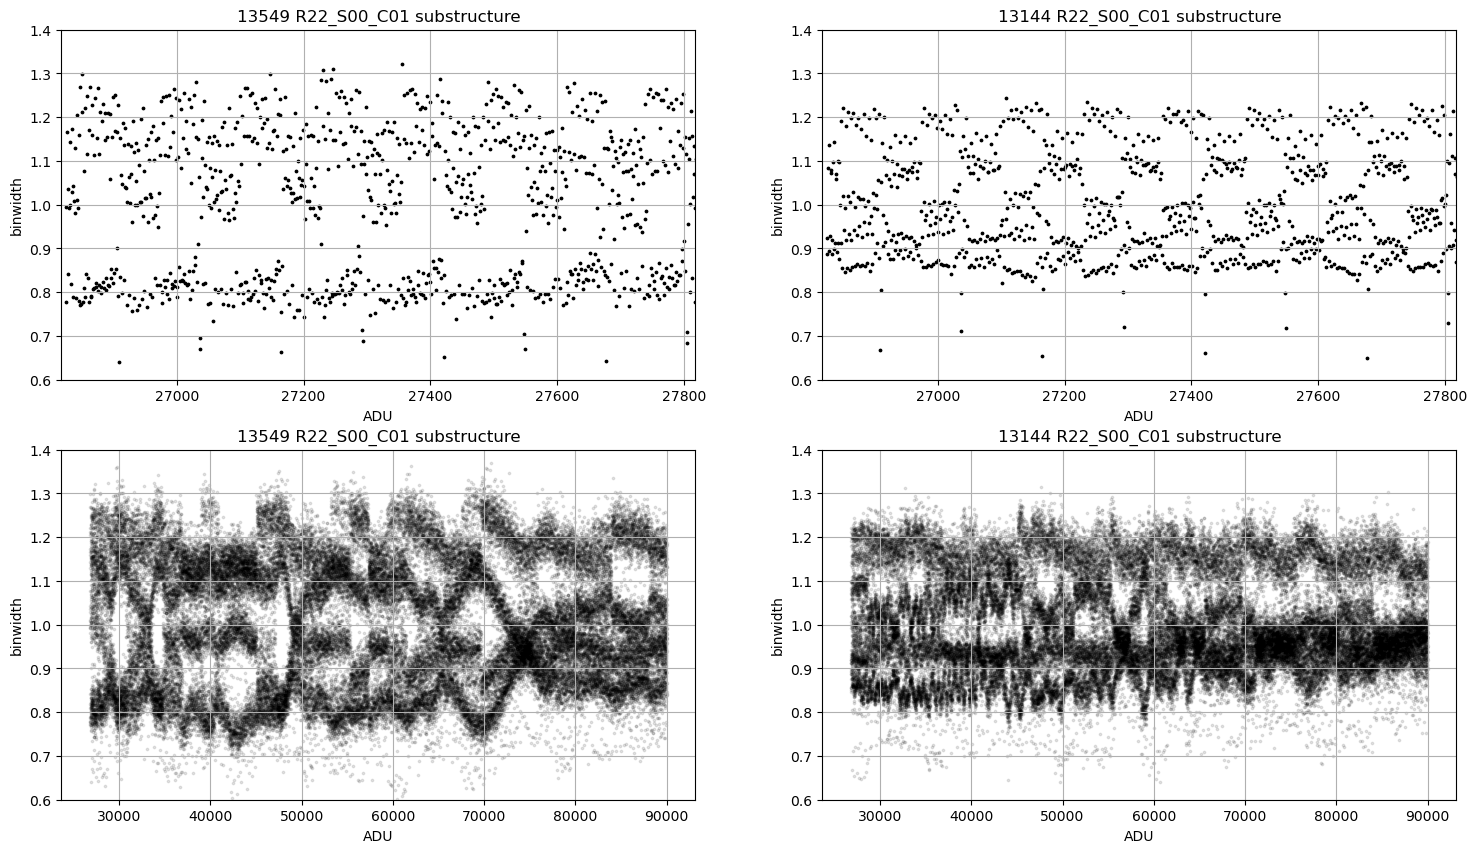
\includegraphics[width=0.75\linewidth]{substructure26825_V2.png}
    \caption{The calibrated bin widths of the the amplifier R22S00C01 from two calibrating runs, 13549 (left column) and 13144 (right column). The full range of calibrated binwidths seen along the bottom row of plots and a zoom version for the earliest ADC bins along the top row. At this zoom level, the substructure of the ADC can be seen. Some slight deviations can be seen between the two runs, due to their individual distributions, but both demonstrate regions of macroscopic grouping of DNL and yield similar bin for bin values of the DNL, as explained in Section \ref{sec:results}.}
    \label{fig:substructureplot}
\end{figure}

Using the ADC calibration process described in Section \ref{sec: Cummulative binning}, we are able to calibrate 3023 of 3024 non-corner ADCs on the LSST Camera focal plane using both runs 13144 and 13549. 
The runs are compared by selecting the first left starting edge for both calibrations to be a bin with suitable information to start the binning process, as described in Sections \ref{sec: SkippedBins} and \ref{sec:Recommended start}.
We will demonstrate the robustness of this method across runs by examining individual substructure, differential nonlinearity, integral nonlinearity, width and edge location differences, and edge location differences as a function of starting bin. 
We then examine the results for the entire focal plane to see how the method does more generally.

\subsection{Substructure}
\label{sec:substructure}

For each individual amplifier’s ADC we can plot the binwidth as a function of ADU as seen in Figure \ref{fig:substructureplot}. 
The plot demonstrates that the spread in binwidths is between (0.65, 1.35) for both calibrations for our sample amplifier. 
This plot also demonstrates macroscopic groupings of binwidths through this calibrated region of the ADC. 
These groupings are repeated throughout the used range of the ADC, seen in the bottom row plots of Figure \ref{fig:substructureplot}, showing that the structure of the ADC is periodic.

Our result also demonstrates that for this amplifier, R22S00C01, there are narrow bins every 128 codes. 
These small bins, or downticks, correspond to the same ADU values where the histogram demonstrated low occupancy, as seen in Figures \ref{fig:13144Distributions} and \ref{fig:13549Hist}.
This actively demonstrates that the method recovers the characteristics of the source distribution. 
This downtick behavior is found in many, but not all, additional amplifiers.
Since the method recovers this fingerprint, we suggest this is an early clue both calibrations do a sufficient job calibrating the ADCs as both have this feature present.

Another notable aspect of Figure \ref{fig:substructureplot} are the slight differences in the binwidth distribution by calibrating run. 
As seen here, there are some differences between the left and right plots, or the exact locations of the edges, stemming from minute differences of the calibrating run.  
This is most clearly seen in the clumping of binwidths for widths greater than 1, while there is good agreement for binwidths less than 1. 
We will explore in Section \ref{sec:Left Differences} the specific edge location differences of the in more detail, but note it here as a structural difference.  

\begin{figure}[t]
    \centering
    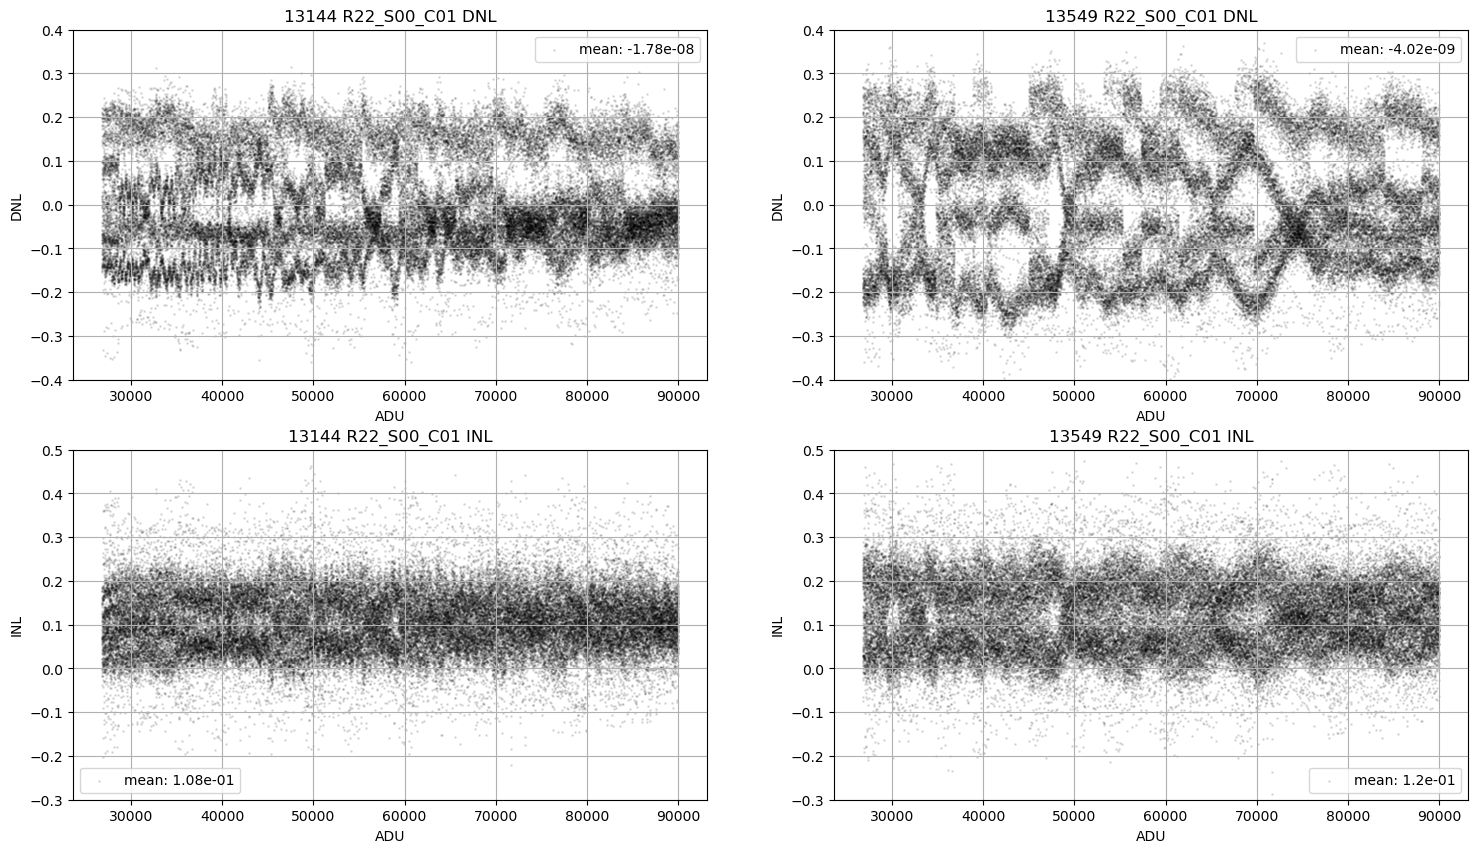
\includegraphics[width=0.75\linewidth]{DNLILN26825_v2.png}
    \caption{Plots demonstrating DNL (top row) and INL (bottom row) for the two calibrating runs, 13144 (left) and 13549 (right) for amplifier R22S00C01. The DNL is strictly between [-0.4, 0.4] for all bins of the ADC when binning commences at the same starting bin, with the mean DNL in both calibrations below 1e-6. The INL remains between [-0.4, 0.5] for all bins of the ADC when binning commences at the same starting bin. Both calibrations yield a mean INL of approximately 0.1.}
    \label{fig:calibratedDNLINL}
\end{figure}

\subsection{Differential Nonlinearity, Integral Nonlinearity}
\label{sec:resultDNLINL}


From Section \ref{sec: DNL_INL_Def}, the calibration of the ADC is dependent on and informed by the presence of DNL within the ADCs. 
Here we examine the degree to which the differential linearity and integral linearity match that of the expectation from their manufacturer. 
We examine this separately for each type of nonlinearity to add validity to the cumulative binning method.

We will first examine the DNL as reported over the ADC for both calibrations. 
In the top row plots of Figure \ref{fig:calibratedDNLINL} we demonstrate the spread of the DNL by ADU. 
For both runs, the DNL is spread over the range (-0.4, 0.4) which falls within the manufacturer's specifications (\cite{AnalogDevices}). 
Additionally, there is good agreement between the two runs, notably in the range of the DNL over all ADC bins. 
More specifically, there are subtle differences in the DNL structure between the two runs, inherently demonstrating the slight differences between the calibration runs' count distribution. 
Yet even with these differences, the mean value of the DNL is comparable over both runs, with values 2.9e-6 and 1.8e-6 for 13144 and 13549 respectively.
Together this suggests our measured DNL is independent of the run used. 

We also examine the INL for both calibration runs in the bottom row of Figure \ref{fig:calibratedDNLINL}.
The INL ranges between (-0.4, 0.4) for all ADU in both calibrations. 
We note the mean value for each run is -6.5e-2 and -1.38e-1 for 13144 and 13549 respectively. 
These values for the INL directly fall below the maximally stated by the manufacturer, suggesting the calibration is recovering the behavior of the ADC (\cite{AnalogDevices}).

\subsection{Edge Placement Differences}
\label{sec:Left Differences}

\begin{figure}
    \centering
    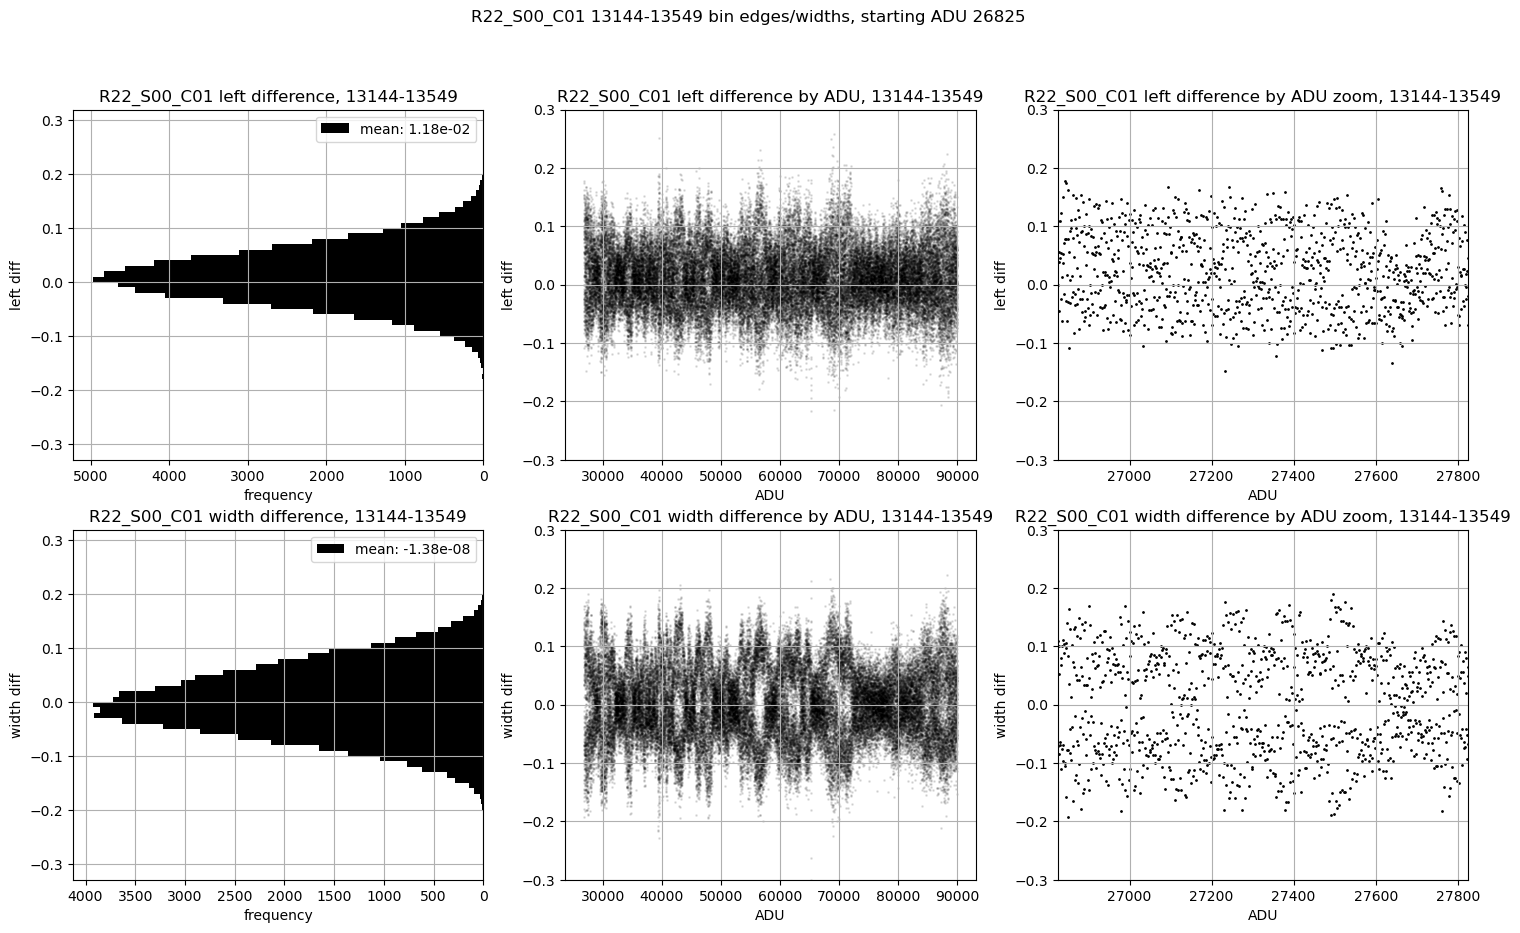
\includegraphics[width=1\linewidth]{calibrationDiff26825.png}
    \caption{The top row demonstrates the left difference of the bin edges 13144-13549 for the sample amplifier R22S00C01. The histogram shows the distribution of this difference, a normal distribution with a mean of 0.0118, with the deviation of such will be examined in Figure \ref{fig:Leftstarting}. The middle top demonstrates these left differences as a function of ADU bin, and the right top plot is a small subsection to demonstrate the spread has no discernible pattern in the left differences. The bottom row demonstrates the same plots for the width difference of each ADC bin: histogram, all ADU, and subregion. We note the histogram is normally distributed about 0 (mean -1.38e-8) and is consistent over the calibrated range of the ADC.}
    \label{fig:leftwidthADU}
\end{figure}

To understand the deviations of the edges by calibrating run, we examine the locations of the left edges and binwidths seen in Figure \ref{fig:substructureplot}. 
We will accomplish this by first looking at the left edge placement difference for each ADU. 
We will then examine differences in the each bin widths by ADU. 
We conclude this section by examining whether any dependence may exist between the starting bin ADU and the left/binwidth differences.  

First we look at the exact edge placement of the left edges of each ADU bin.
This choice is motivated by the method, in that we place the first left edge for both calibrations at the same ADU.  
The left difference is determined by running the calibration on both runs starting from earliest selected bin as described in Section \ref{sec:Recommended start}, then subtracting one set of left edges from the other, specifically the ramp determined edges from flat pair determined edges. 
The result of such a method is shown in Figure \ref{fig:leftwidthADU}. 
The distribution of left edge differences is shown in the top row. 
The plot demonstrates the left differences themselves, bin to bin, form a normal distribution centered around its mean -0.07, the leftmost plot. 
We see that the left edges differ between (-0.3, 0.2).  
This means on average that the bins from the ramp run calibration, 13549, are slightly larger on average than that of the bins from the rescaled flat pairs 13144 for this amplifier when binning starts on the earliest possible bin.
We attribute this difference due to the forced estimation of the first left edge to be somewhere in the distribution. 
That is, the first placed ADU bin edge may not exactly be where we place it, but without a prior information about the location of the bin edges, the method must begin somewhere. 
We will further examine this nonzero deviation of the mean later in Figure \ref{fig:Leftstarting}. 
Looking at the center and rigthmost plot of the left difference, we note the lack of structure when examining left difference as a function of ADU bin.
This suggests that the two edges clearly follow each other throughout the calibrations and the mean deviation is systematic. 

Doing a similar analysis, but instead subtracting the widths of each distribution by ADU code, we can examine how well the two runs calibrate the binwidths themselves. 
This is plotted as the bottom row of Figure \ref{fig:leftwidthADU}.
The width differences themselves have a mean of -1.8e-6, and are also normally distributed as seen in the leftmost plot.
They feature a range of binwidth difference between(-0.2, 0.2) over the calibrated ADC bins. 
When plotted by ADU, the width difference makes no discernible pattern in near or long-term visualizations, seen in the middle and rightmost plots. 
This suggests the method is robust in calibrating the binwidths, and the binwidths closely follow from one calibration to the other. 

To further check for differences in the calibrations, we examine the potential impact of the first starting left edge on the left edge difference and the binwidth difference. 
In Figure \ref{fig:Leftstarting} we plot the left edge difference as a function of ADU as a function of starting ADU value for 1000 successive ADU values. 
Not included is the width difference dependence, due to its negligible mean difference on the order of 1e-6 as shown in Figure \ref{fig:leftwidthADU} for all starting ADU.
The plot demonstrates there is some variation of the left edge difference as a function of the starting bin.
The mean left differences sits between (-0.15, 0.15) over 1000 successive bin starts, with a mean of these means of 0. 
This verifies that there is some dependence on the calibration based on where the first left edge is placed, but the deviation on average is less than $|0.2|$ regardless of starting bin, suggesting the method does a sufficient job for both calibrations to align. 

\begin{figure}
    \centering
    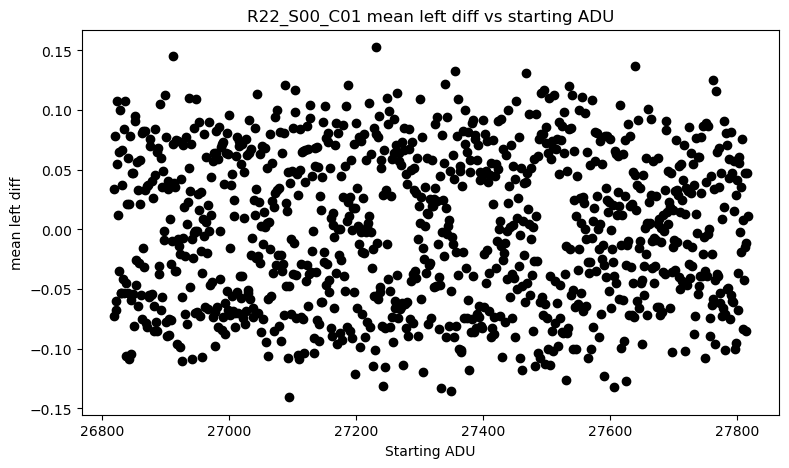
\includegraphics[width=0.5\linewidth]{meanleftbyADU.png}
    \caption{The mean left difference between the two calibrating runs as described in Section \ref{sec: Cummulative binning} by starting ADU. From Figure \ref{fig:leftwidthADU} there is a non zero mean difference of the left edges over for the calibrated ADC bins. The mean left difference is dependent on the starting ADU selected to commence binning. The difference in left edge placement is within the range of [-0.15, 0.15], with a mean of 6e-5 depending on selected starting ADU.}
    \label{fig:Leftstarting}
\end{figure}


\subsection{Focal Plane}
\label{sec:Focal Plane}

\begin{figure}
    \centering
    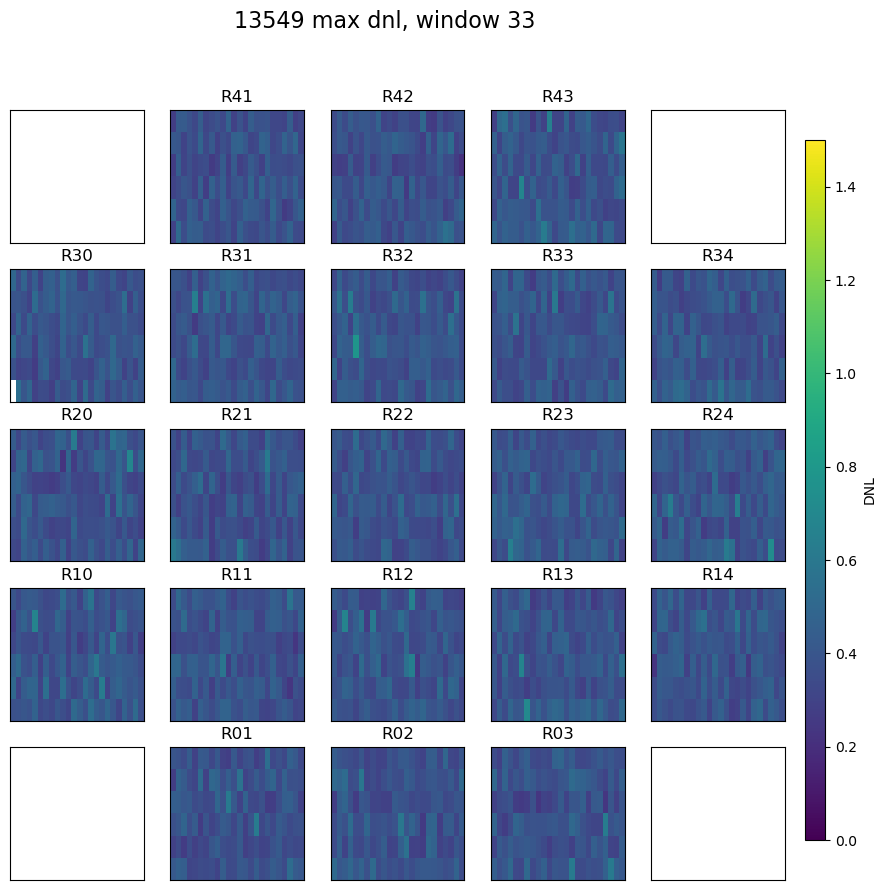
\includegraphics[width=0.75\linewidth]{maxdnl13549.png}
    \caption{The absolute value maximum DNL as computed for every ADC bin when calibrated via the method we described in Section \ref{sec:PDFEdges}. This method computes edges along the ADC for each 3023 amplifiers individually for the ramp run (13549). The DNL is computed for each bin, in each amplifier, and maximum magnitude DNL of all bins is plotted. Value of maximum magnitude DNL ranges between 0 and 1 for all ADCs shown.}
    \label{fig:focalplaneDNL}
\end{figure}

\begin{figure}
    \centering
    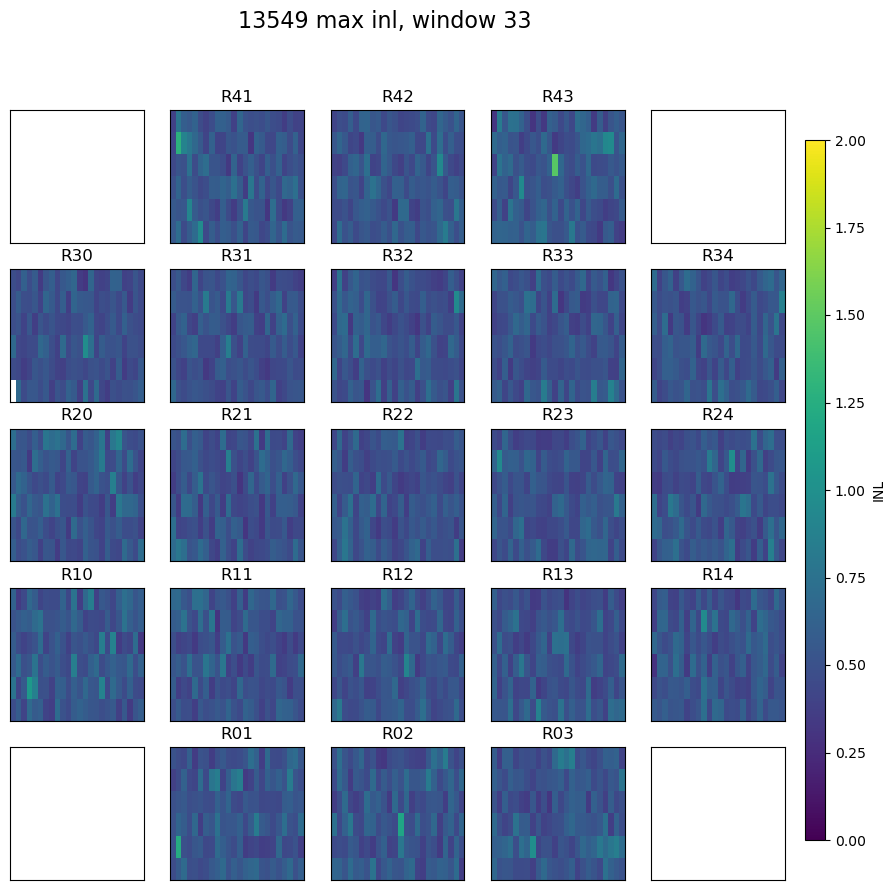
\includegraphics[width=0.75\linewidth]{maxinl13549.png}
    \caption{The absolute value maximum INL as computed for every ADC bin when calibrated via the method we described in Section \ref{sec:PDFEdges}. This method computes edges along the ADC for each 3023 amplifiers individually. The INL is computed for each bin, in each amplifier, and the maximum magnitude INL of all bins is plotted. Values range between 0 and 2, and are below the maximally allowed by the ADC manufacturer.}
    \label{fig:focalplaneINL}
\end{figure}

Beyond a single amplifier, we can further look at the entire focal plane, and the edges made for each of the ADCs. 
For the sake of space, we show just the calibration of 13549 over the entire focal plane. 
We can examine the maximally achieves DNL and INL for this run to verify whether all calibrated ADCs fall within specifications and behave as expected. 
We will also examine the mean left edge difference and the mean width difference between the two calibrations for all calibrated ADCs. 

Figure \ref{fig:focalplaneDNL} demonstrates the absolute value maximum DNL for all bins for every ADC on the focal plane. 
The DNL falls within the allowable 0.85-1.5 range as set by the manufacturer (\cite{AnalogDevices}).  
This suggests the calibration method is representing the DNL accurately and matches that of the device specifications. 
Figure \ref{fig:focalplaneINL} demonstrates the absolute value maximum INL for all bins for every ADC on the focal plane. 
The INL falls within $\pm$ 2 for every ADC. 
This suggests we have all the ADCs within the specifications set by the manufacturer. 
We also see the same result came from 13144 as well, although plots are not included. 
We note here that two amplifiers for 13144 did not have sufficient data, R03S11C00 and R30S00C10 and are exclude from calibration. 
R30S00C10 is also excluded from 13549 and is seen as a blank amplifier in Figures \ref{fig:focalplaneDNL} and \ref{fig:focalplaneINL} due to the same terminated dataset issue.
We note that both these amplifiers have been previously characterized as dead amplifiers, and more information on them is detailed in Table 7 of SitCom 148 from The LSST Camera group, Antilogus, et al. in prep (\cite{Antilogus2025}).

To further illustrate the strength of this calibration, we plot the mean width difference for every amplifier. 
In this, we calculate the width difference for every bin between the two calibrations as shown in Figure \ref{fig:leftwidthADU}. 
We then compute a mean for each amplifier, and plot all those means together as the left plot of Figure \ref{fig:focalplanehistograms}. 
The results demonstrate the mean binwidth differ by run on is on average near 0, with deviations on the order 1e-5. 
This suggests the width calibration is very robust from one calibration run to another. 


We also examine how the left edges deviate from one run to the other for all calibrated ADCs.
We first calculate the difference in the location of the left edges between the two calibrations as seen in Figures \ref{fig:leftwidthADU}. 
We then compute the mean of this left edge difference, and plot as a histogram for all the calibrated amplifiers seen as the right plot of Figure \ref{fig:focalplanehistograms}. 
This result demonstrates that the average mean left edge difference is 0, with a range of [-0.4, 0.4]. 
This furthers our conclusion from Section \ref{sec:Left Differences} that suggests the exact location of the first left bin dictates how well the two calibrations match. 
That is to say, there is less than a 0.5 difference between calibrations depending on how well the first left edge is placed. 

We importantly note, there is no dependence on the calculated INL and DNL as a function of starting ADU. 
This is discussed more in detail in the appendix, as this was an early motivator for this work. 
This implies we are able to calibrate the ADC regardless of the commencing bin, and any minute issues with placing the first left bin does not propagate into DNL and INL measurements. 
This suggests that using a pre-scale on a flat pairs run works just as well for this DNL calibration of the ADC as using a ramp run. 

\begin{figure}
    \centering
    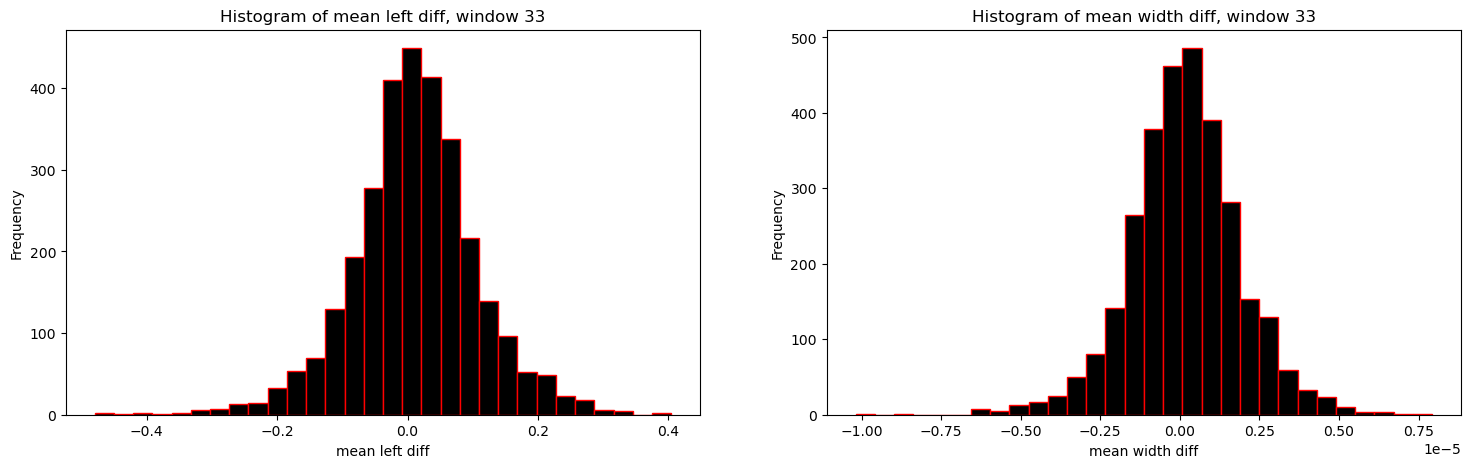
\includegraphics[width=1\linewidth]{meandifferencehist.png}
    \caption{The left(right) plot is a histogram of the mean left(width) difference for each amplifier calibrated using the method described in Section \ref{sec: Cummulative binning}. The value reported here is representative of the mean shown in Figure \ref{fig:leftwidthADU}, of the left(width) difference between the two calibration runs by ADU. The distribution of these means are normal with the average difference of 1.9e-2(2.3e-7), spread of deviations of the between [-0.5, 0.5]([-1e-5,1e-5]).}
    \label{fig:focalplanehistograms}
\end{figure}

\section{Discussion}
\label{sec:Future}

The work presented in this paper outlines the ability to calibrate each of the LSST Camera's ADC on the focal plane.
The results of such calibration demonstrate both DNL and INL within the specifications set by the manufacturer (\cite{AnalogDevices}).
We note the ADCs appear to be stable, as the comparable results of the edge placements, binwidths, DNL, and INL values per bin between the two calibrations, 13144 and 13549. 
This stability is also through time, as  the exposures in the runs were taken in December 2021 and November 2023 (13144 and 13549 respectively).

More generally, this method serves as a method to calibrate any ADCs. 
As projected in Figure \ref{fig:idealADC}, this method allows the conversion of bin edges from integer to real values, allowing for greater precision in measurements.
We include a truncated version of a look up calibration table for our sample amplifier as an example in Table \ref{tab:Table1}.
We note that we subtracted a pedestal of 26825 to align these values with zero for ease of comprehension.
The table provides the specific two edges corresponding to the given ADU, or the x axis of Figure \ref{fig:idealADC}. 
A recreation of the ideal plot can be seen as Figure \ref{fig:1314413549Edges}, where the edges of ADC are shown in red from the flat pairs (13144) and black from the ramp (13549). 
The differences discussed in Section \ref{sec:results} can be seen explicitly. 

Seen in this work, the differences between the calibrations are the result of  the calibrating run for the ADCs. 
Based on our results, we recommend any calibration of ADCs be completed using a ramp equivalent method. 
We recommend this due to the need to heavily rescale flat pair data in order to find a suitable ADC calibration, although both show good agreement in edge placement after such a rescale is completed. 

We reiterate here that this work demonstrates a calibration method for any general ADCs, with LSST Camera as the focal point and its results shown explicitly. 
Our method demonstrates great consistency between two calibrating dataset types in terms of binwidths, DNL, INL, and we provide a sample calibration look-up table for clarity. 

\begin{table}[h]
    \centering
    \begin{tabular}{|c|c|c|}
        \hline
        ADU & 13144 & 13549 \\
        \hline
        0 & 0, 0.888 & 0, 0.778 \\
        1 & 0.888, 1.812 & 0.778, 1.773 \\
        2 & 1.812, 2.895 & 1.773, 2.94 \\
        3 & 2.895, 4.031 & 2.94, 3.975 \\
        4 & 4.031, 4.926 & 3.975, 4.817 \\
        5 & 4.926, 5.854 & 4.817, 5.809 \\
        \hline
    \end{tabular}
    \caption{The first few ADU codes as calibrated from the ADC from the cumulative binning method described in Section \ref{sec: Cummulative binning}. This is a numeric version of Figure \ref{fig:substructureplot}, demonstrating real value placement of the edges of the ADC. We represent the numeric value of the (left edge, right edge) for both calibrating runs. These value have a subtracted pedestal of 26825, which is the true first edge placed by the method. We see good agreement but slight differences between the two calibration runs as noted in Sections \ref{sec:results} and \ref{sec:Future}.}
    \label{tab:Table1}
\end{table}

\begin{figure}
    \centering
    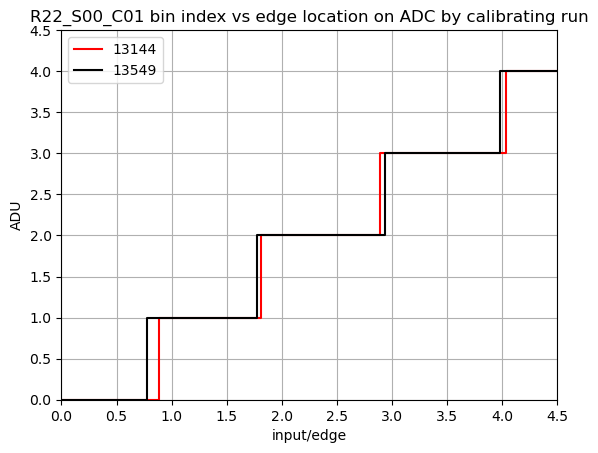
\includegraphics[width=0.5\linewidth]{TrueADCEdges.png}
    \caption{The exact bin edges of calibrating runs 13144 (blue) and 13549 (orange), and how they correspond to ADU. The values are normalized by the starting bin for this amplifier, 26825, as seen in Table \ref{tab:Table1}. }
    \label{fig:1314413549Edges}
\end{figure}




\begin{acknowledgments}
The authors would like to thank Yousuke Utsumi for helpful comments on an early version of this draft. We also thank the entire LSST Camera team for feedback while this work was ongoing. This work is funded by.
\end{acknowledgments}

\bibliography{references}{}
\bibliographystyle{aasjournalv7}

\appendix

The following appendices serve as additional details to some effects mentioned earlier in this work. 
These notes are to aid future ADC calibrations wishing to follow this work. 
Appendix \ref{sec:Adrianmethod} details an early simplified ADC calibration. 
Discussion of where to examine the ADC DNL is covered in discussion of bit fractions in Appendix \ref{sec: BitFractions}.
Appendix \ref{sec:Dynamic Prescaling} details an alternative scaling method to the rolling scaling introduced in Section \ref{sec:RollingScaling}. 
Appendix \ref{sec:OtherFilters} discusses additional filters which could be used to model the no DNL ADC. 
Finally, Appendix \ref{sec:Convergence Interval} discusses the importance of the convergence integral for determination of the ADC bin edges as discussed in Section \ref{sec:PDFEdges}. 

\section{First Pass DNL ADC Calibration}
\label{sec:Adrianmethod}

This section details the preliminary DNL informed ADC calibration by A. Shestakov, which inspired the work described in Section \ref{sec: Cummulative binning}.
The calibration uses run 13144, as shown on the left of Figure \ref{fig:13144Distributions}, and applies a Savitzky-Golay w65o3 to model an ideal ADCs behavior. 
An approximate DNL for each bin was then computed, using the a tentative definition of the DNL  
 \begin{equation}
 DNL = \frac{f_i}{c_i}
 \label{eq:dnlfrac}
 \end{equation}
where the $f_{i}$ is the expected number of counts from the filter, and $c_{i}$ is the observed number of counts from the true distribution for the ADC bin. 
Equating equation \ref{eq: DNL} with equation \ref{eq:dnlfrac} we yield an equation for the widths along the ADC as
 \begin{equation}
 w = 1-DNL = 1- \frac{f_i}{c_i}
 \end{equation}
Assuming the first left edge correspond to the first ADU with signal, the edges of the bins were placed accordingly as
 \begin{equation}
r = l + w 
\end{equation}
where r is the right edge and l is the left edge. 
This allowed the calibration of the ADC over a range of approximately 26-100k ADU, which is roughly bias through saturation of the CCD.  

This method yields a calibrated ADC where both INL and DNL have deviations from specification. 
Here we will break down the nonlinearities independently to parse where they come from in this calibration. 
The left side of Figure \ref{fig:originalDNLINL} demonstrates the DNL as computed using this method from earliest possible bin. 
One can clearly see that for low ADU there are many large, greater than $|0.5|$ ADU DNLs, yet later on the DNL falls within a more expected values. 
This translated into early bin widths being very narrow while later bins are much wider. 
We break the reasoning for this phenomena into two parts. 
The first is the indication that the filter itself struggles to characterize a true ADC for low ADU.
That is the $f_{i}$ are small on average early on as compared to the data point they are fitting.
This can be explicitly shown by plotting the w65o3 filter onto the histogram itself. 
This issue disappears when the filter starts beyond the peak near bias, suggesting there is a distribution based issue for the filter fitting the data accurately, an issue we will examine closely in Section \ref{sec:Filter}.

There is also structure in the INL resulting from this method described in Section \ref{sec:Adrianmethod}.
The right plot in Figure \ref{fig:originalDNLINL} demonstrates unbounded INL over the range of the ADC used, with a maximum deviation of over 140 ADU. 
Clever cuts to the distributions successfully lowered INL contributions to 10 ADU, but reduced the scope of the calibration significantly to cover a range of about 30,000 ADU. 
This suggested that no amount of clever cuts would be able to coax both the INL and DNL into specifications. 

Another notable dependence arose between the starting bin and the maximum magnitude INL contribution achieved over the calibration. 
It is noted, but not shown, that a shift of 1 ADU in starting location could result in maximum INL change of over 100 over the range of the calibration ADU codes. 
The would suggest that the starting location in ADU was highly dependent on the calibration returned by this early method, an instability which is detrimental for robust calibrations. 
Together these issues with INL and DNL indicated the need for a more robust treatment of the calibration method, which we develop in this work. 

\begin{figure}
    \centering
    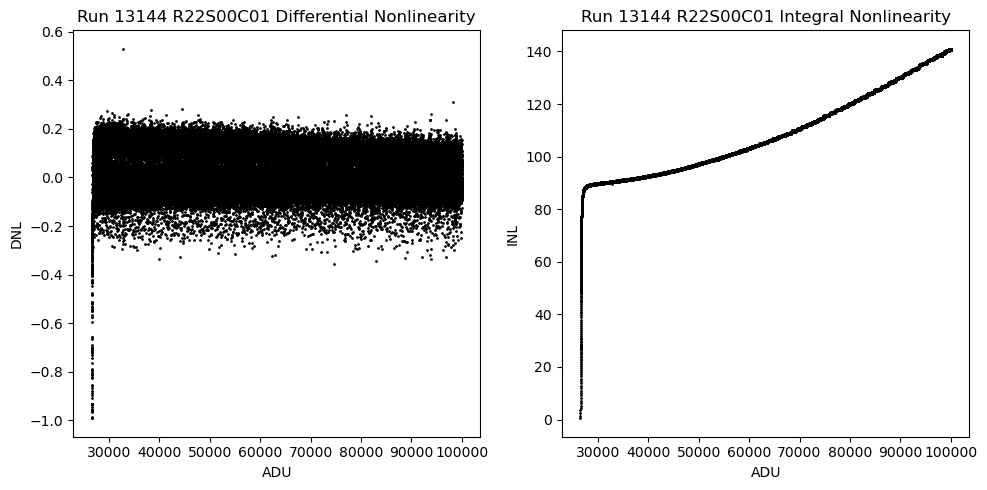
\includegraphics[width=1\linewidth]{OldINLDNL.png}
    \caption{The left plot demonstrates the contributions to the differential nonlinearity using the method described in Appendix \ref{sec:Adrianmethod} for amplifier R22S00C01. For sub 30000 ADU, the DNL sharply peaks, while the DNL stabilizes for higher ADU. On the right is a plot of the unbounded integral nonlinearity that grows progressively throughout the flux range of the CCD, first sharply for low ADU then more gradually for higher ADU.}
    \label{fig:originalDNLINL}
\end{figure}

\section{Bit Fractions}
\label{sec: BitFractions}

In this section, we motivate the use of the rescaling the flat pairs run, 13144, on order of 100 and use of the Savitsky-Golay filter's window size of 33 in our method. 
We will examine both these claims by examinging a quantity we term "bit fraction". 
The bit fraction is a representation of how often a specific bit, as the binary representation of an ADU code, is turned on. 
In an unbiased ADC, we would expect that the bit fraction is exactly 0.5 for all bits. This corresponds to an even amount of times where the bit is turned on and turned off. 
We calculate the bit fraction as the following: 
\begin{equation}
b_x = n_x/N 
\label{eq:bitfract}
\end{equation}
where $b_x$ is the bit fraction for the xth bit, $n_x$ is the number of times this bit is turned on, and N is the total number of codes examined. 
We could examine this fraction for all 18 bits of our ADCs, but choose to limit our examination for this paper to bits 0-7 to examine the range of 0-128. 
This range is suitable for our rescaling region and our filter window. 

We first examine our need to rescale the flat pairs, 13144, in window sizes of 100.
To do this, we compute the bit fractions for the unscaled 13144 and compare to the ramp run 13549. 
The bit fractions are computed for bits bits 0-7 as in Figure \ref{fig:Tworunbitfrac}. 
Examining that figure, we see that for the ramp run, 13549, bits 0 and 1 are the least well behaved, with no notable excursions beyond these two bits. 
We note that the behavior is different for the unscaled flat pairs, 13144. 
We note some excursions seen in bits 6 and 7, which are not present in the ramp run.
We interpret this result to being inherent to the data taking, rather than the ADC as if a characteristic of the ADC it should be seen in both runs.
We further use this to justify the use of rescaling in the flat pairs to see the true behavior of the ADC rather than a print through of the data taking method.
Since there is no notable bit fraction deviations beyond the 2 least significant bits (LSB), we can scale our data well outside this window and use 100 as this window size in the calibration. 

In Figure \ref{fig:Singleampbitfrac} we seek to examine if a regional dependence of the bit fractions exists for the ramp run 13549. 
We select doing this analysis on the ramp run to avoid issues with data shape impacting our bit fractions, as noted earlier the data shape impacts which ADC codes are more/less represented. 
The plot demonstrates for all regions of the CCD, the 2 Least Signficant Bits (LSB) are the least well behaved, and we note no regional dependence exists in the bit fractions. 
This illustrates the well behaved nature of the ADC beyond the 2 LSB. 
We note that for the 0s exposure we do not plot the bit fractions for bits 7 due to poor sampling. 
This allows us to select the window size of 33 to be well beyond the local DNL we wish to measure and recover in the method, and use it in our filter to model an ideal ADC.
We note, but do not explicitly show, that this result of the 2 LSB being the least well behaved is robust over all examined amplifiers shown in this work. 

\begin{figure}
    \centering
    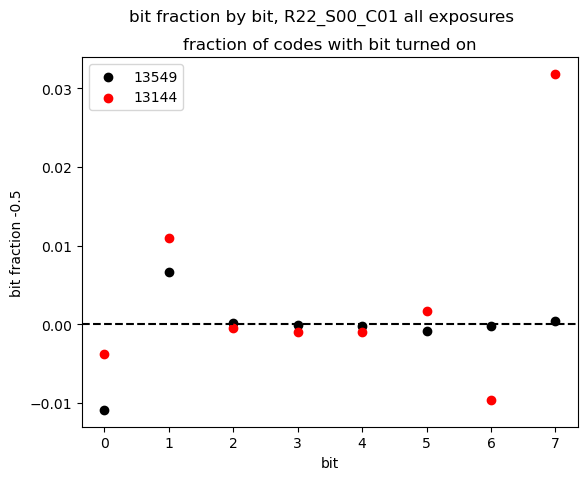
\includegraphics[width=1\linewidth]{bitfractdistr.png}
    \caption{The bit fractions 0-7 along all exposures for two runs 13549 (black) and 13144 (red) for sample amplifier, R22S00C01. The two LSB are the least well behaved over the range of the ADC examined for both runs. The flat pairs, 13144, demonstrate poor behavior and deviation from 0 bit fraction in bits 6 and 7. Since this behavior is not also seen in the ramp run, this can be attributed to the nonuniform scaling in the flat pairs, as if it were true behavior of the ADC it would also be present in the ramp run, 13549.}
    \label{fig:Tworunbitfrac}
\end{figure}

\begin{figure}
    \centering
    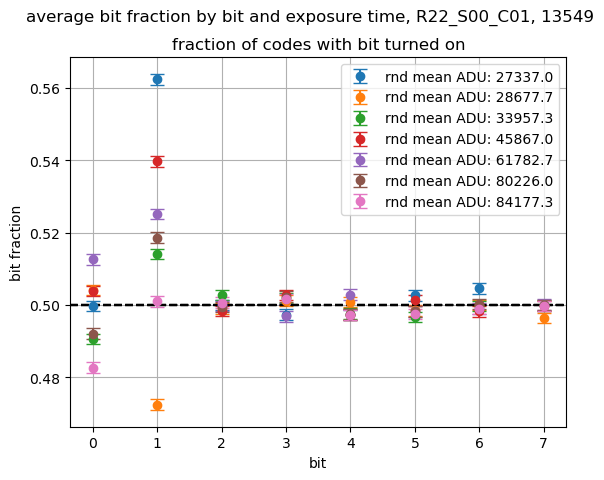
\includegraphics[width=1\linewidth]{bitfracterr.png}
    \caption{The bit fractions as calculated for 6 various exposure times between 0 and 94.6 seconds from ramp run 13549, to probe whether a regional dependence to the bit fractions exists for our sample amplifier R22S00C01. The legend specifies the mean rounded ADU of the data point represented. The two LSB are the least well behaved for all regions of the ADC probed, with deviations from 0 in their bit fractions. The bit fraction for bit 7 and 0s exposure time is not included due to poor sampling in that region. Error bars represent 95 percent confidence interval on the bit fraction.}
    \label{fig:Singleampbitfrac}
\end{figure}


\section{Dynamic Prescaling Flat Pairs}
\label{sec:Dynamic Prescaling}


Before developing the rolling scaling method  used in Section \ref{sec:RollingScaling}, we used a dynamic prescaling factor reduce the amount of data in the low flux region while preserving use of all exposures in the flat pairs run.
In practice we examine the region of the ADC where the combined signal is relatively flat, typically higher ADU codes, and select the saturation level for the entire distribution. 
For run 13144 we used 5000 counts per ADU was sufficient. 
We then compute a prescale factor, $\chi _i$, for each 25 ADU subregion of the ADC, where
\begin{equation}
\chi_i = \frac{5000}{c_{av}}
\label{eq: prescale}
\end{equation}
where $c_{av}$ is the average observed counts from the combined histogram over the subregion. 
For any regions of the ADC where the $c_{av} < 5000$ the pre-scale factor was taken to be 1, or all data in that flux region was used for the combined distribution. 

Each exposure is then pulled and its peak signal in ADU is matched with the corresponding pre-scale factor. 
Then the number of samples to select from that exposure, denoted as $\eta $, is determined via
 \begin{equation}
 \eta = \chi_i *n 
 \label{eq:selectedsamples}
\end{equation}
Where the number of pixels in the amplifier, n, is dependent on the type of CCD attached to that ADC, either an E2V or ITL from the two manufacturers of the CCDs which have slightly different numbers of pixels per chip. 
A randomization process selects $\eta$ pixel digitizations from the exposure, and these are added to the combined distribution. 
This is repeated for each exposure in the run, and builds a pseudo-flat distribution over the full flux range of the CCD. 
This method worked sufficiently well, but was abandoned in favor of the rolling scaling used in Section \ref{sec:RollingScaling} for its ease and reduced computation time.

\section{Filter Choices}
\label{sec:OtherFilters} 

We examined the use of many filters to determine Savitzky-Golay w33o3 was the best choice to use in this method. 
Our goal was to find a filter which represents the data clearly over the flux range of the CCD. 
Early work demonstrated the filter tends to undervalue peaked regions, as alluded to in Appendix \ref{sec:Adrianmethod}. 
Thus we examine many filters, windows and order of fit to understand this relationship clearly. 
We compared various filters to our data as well as fabricated data using a chi square goodness of fit. 
We used the following types of filters in our tests; Savitzky-Golay: windows 25-100, 2nd and 3rd order polynomials, and Butterworth: highpass, lowpass, and bandpass. 
The results demonstrated that the Savitzky-Golay filter with window size 33 and order 3, represented all the data examined very well, and was therefore chosen for use in the method.  
As an additional comment, a smaller window size  such as 13, 17, and 19, would allow one to more carefully probe lower order DNL and potentially recover a calibration closer to the bias.  
We found success with these smaller windows, but do not implement them due to an abundance of caution regarding masking out higher order DNL by the smaller window. 

\section{Convergence Interval}
\label{sec:Convergence Interval}


In this section we discuss the work done to evaluate the convergence interval used in the cumulative sum binning method. 
The method uses a convergence interval of $\pm$ specified value to converge on the right edge of the ADC bin, that is the degree to which equation \ref{eq:splineright} is exact.
To quantify this in a more exact way, we include this convergence interval, $\sigma$, into equation \ref{eq:splineright}. 
\begin{equation}
\zeta(r) \pm \sigma = c_i + \zeta(l)  
\label{eq:splinerighterr}
\end{equation}

Through many iterations, we determined a decrease in $\sigma$ corresponded to an increase in computation time.  
For reasonable $\sigma$ values, we found no positive impact on the DNL or INL seen in the distribution. 
Thus, the convergence interval of 1 count optimizes the computation time while still yielding a 0.2 percent difference between the average observed counts and that achieved by the method. 
This difference is very precise with an uncertainty of any single bin average 1/3000, which is significantly lower than other errors which may occur.  

We also examined the result of the convergence integral, or the residual, to see whether this amount was significant in some way. 
In this, we tested whether the residuals had some pattern to them over the range of used ADU codes in the ADC.
It was determined that the residuals make no noticeable pattern over the range of  ADU, and rather also suggests that the bins were not larger or smaller than expected. 
Thus we ruled out that the uncertainty of 1 count was sufficiently low, while maximizing the computation time for all bins of a single ADC in under 30s. 

We also tested adding the residual to the next bin, as an ad hoc method of dealing with the residuals. 
The results of such calibration found no noticeable changes in the DNL.
Yet new structure emerged in the INL, suggesting adding the residuals caused misplacement of the next adjacent bin. 
This can be understood by thinking of adding the residual changing the next bin size, and iterating over 100k bins, resulting in an extreme case with over 100k counts, which will affect where the bin edge will be placed.
These changes, coupled with 0.2 percent difference suggests the residuals were of a negligible amount and no more robust treatment of them is necessary. 

\end{document}